% begin module tangent-problem
\begin{frame}
\begin{columns}[c]
\column{.4\textwidth}
\psset{xunit=1cm, yunit=1cm}
\begin{pspicture}(-5, -5)(5,5) 
\psframe*[linecolor=white](-5,-5)(5,5) 
\tiny
\psaxes[ticks=none, labels=none]{<->}(0,0)(-1.05,-0.52)(3.1,4.2)
\psLabelsWithOnes{3}{4.2}
\rput(-0.35,0.6){$y=x^{2}$} 
%Function formula: (x)^{2} 
\psplot[linecolor=red, plotpoints=1000]{-1}{2}{x 2 exp }
\psFullDot{1}{1}
\rput[lt](1.1,1){$P=(1,1)$}

\uncover<-5>{
\psline[linecolor=blue]( 0.25,-0.5)(2.55 ,4.1)
}
\uncover<7-8>{
\rput[lt](2.1,4){$Q=(2,4)$}
\psFullDot{2}{4}
\psline[linecolor=blue]( 0.5,-0.5)(2.033333333 ,4.1)
\psLabelNumberXYaxes{2}{4}
}
\uncover<9-10>{
\rput[lt](1.6,2.25){$Q=(1.5,2.25)$}
\psFullDot{1.5}{2.25}
\psline[linecolor=blue]( 0.4,-0.5)(2.24 ,4.1)
\psLabelNumberXYaxes{1.5}{2.25}
}
\uncover<11-12>{
\rput[lt](1.35,1.5625){$Q=(1.25,1.5625)$}
\psFullDot{1.25}{1.5625}
\psline[linecolor=blue]( 0.333333333,-0.5)(2.377777778 ,4.1)
\psXYTick{1.25}{1.5625}
}
\uncover<13-16>{
\rput[lt](1.2,1.21){$Q=(1.1,1.21)$}
\psFullDot{1.1}{1.21}
\psline[linecolor=blue]( 0.285714286,-0.5)(2.476190476 ,4.1)
\psXYTick{1.1}{1.21}
}
\uncover<17-18>{
\rput[lt](0.1,0){$Q=(0,0)$}
\psFullDot{0}{0}
\psline[linecolor=blue]( -0.5,-0.5)( 2.95,2.95)
}
\uncover<19-20>{
\rput[lt](0.6,0.25){$Q=(0.5,0.25)$}
\psFullDot{0.5}{0.25}
\psline[linecolor=blue]( 0,-0.5)( 3.066666667,4.1)
\psXYTick{0.5}{0.25}
}
\uncover<21-22>{
\rput[lt](0.85,0.5625){$Q=(0.75,0.5625)$}
\psFullDot{0.75}{0.5625}
\psline[linecolor=blue](0.142857143 ,-0.5)( 2.771428571,4.1)
\psXYTick{0.75}{0.5625}
}
\uncover<23->{
\rput[lt](1,0.81){$Q=(0.9,0.81)$}
\psFullDot{0.9}{0.81}
\psline[linecolor=blue](0.210526316 ,-0.5)(2.631578947 ,4.1)
\psXYTick{0.9}{0.81}
}
\end{pspicture} 
%\ \only<handout:1| -5>{%
%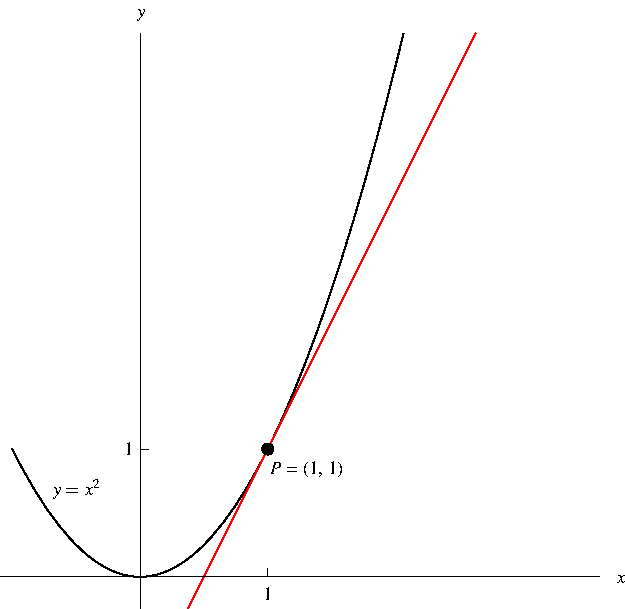
\includegraphics[height=5cm]{limits/pictures/02-01-secanta.pdf}%
%}%
%\only<handout:0| 6>{%
%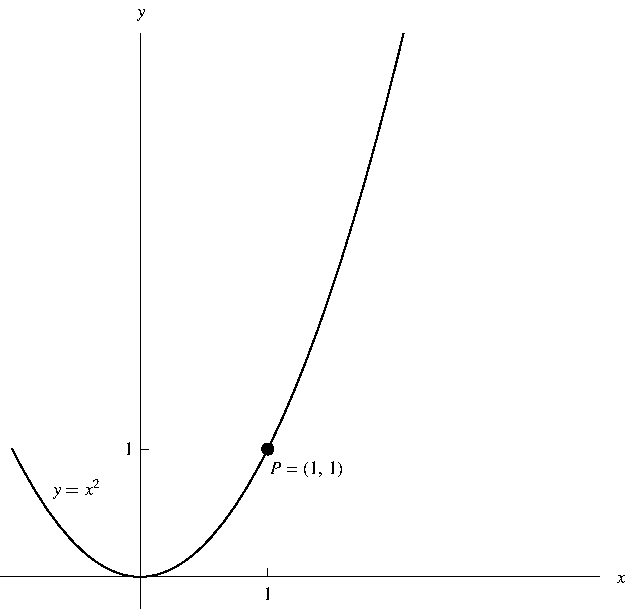
\includegraphics[height=5cm]{limits/pictures/02-01-secantb.pdf}%
%}%
%\only<handout:2| 7-8>{%
%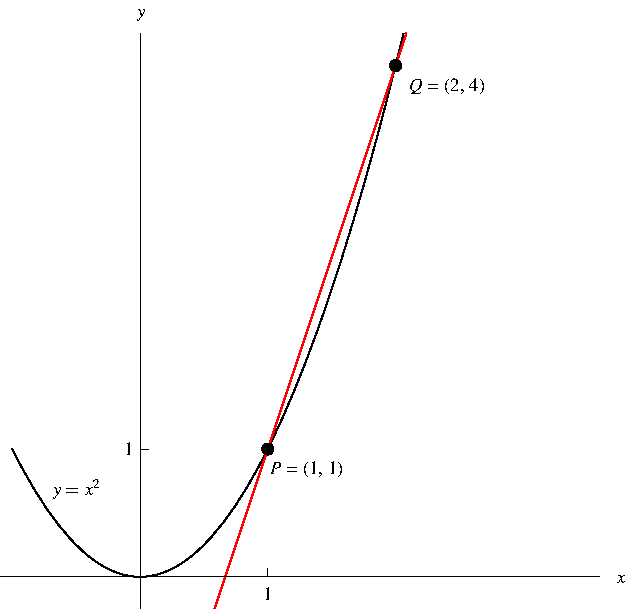
\includegraphics[height=5cm]{limits/pictures/02-01-secantc.pdf}%
%}%
%\only<handout:0| 9-10>{%
%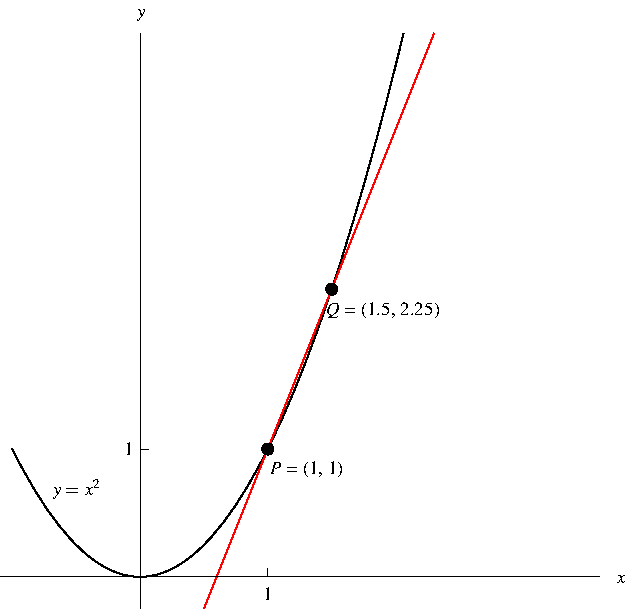
\includegraphics[height=5cm]{limits/pictures/02-01-secantd.pdf}%
%}%
%\only<handout:0| 11-12>{%
%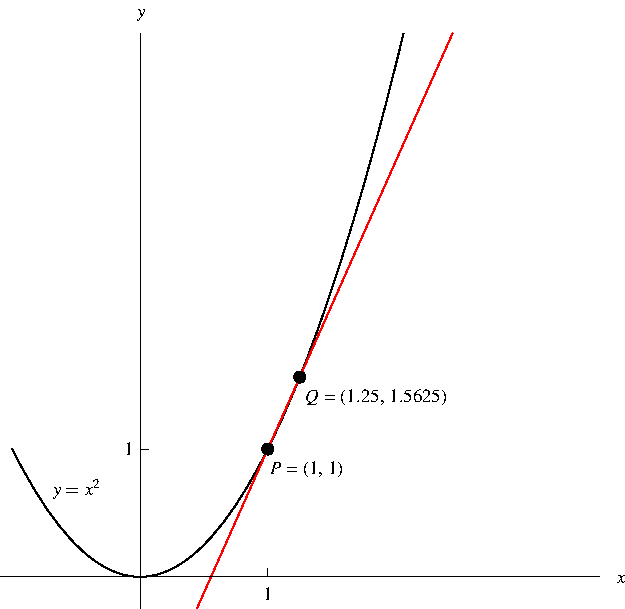
\includegraphics[height=5cm]{limits/pictures/02-01-secante.pdf}%
%}%
%\only<handout:0| 13-16>{%
%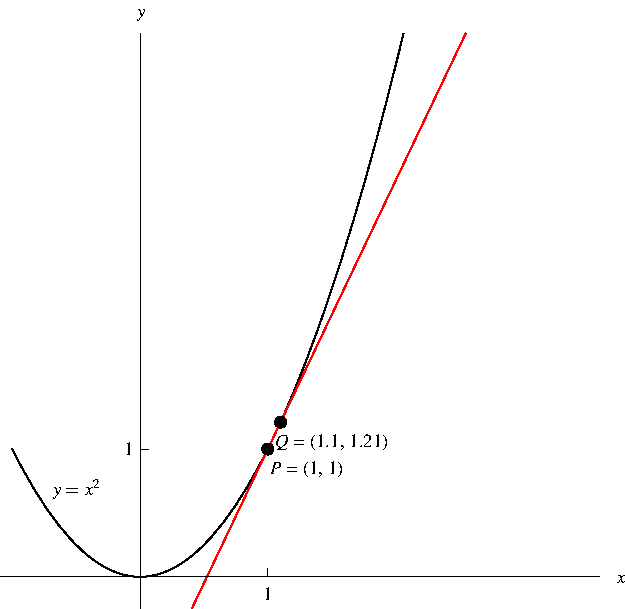
\includegraphics[height=5cm]{limits/pictures/02-01-secantf.pdf}%
%}%
%\only<handout:0| 17-18>{%
%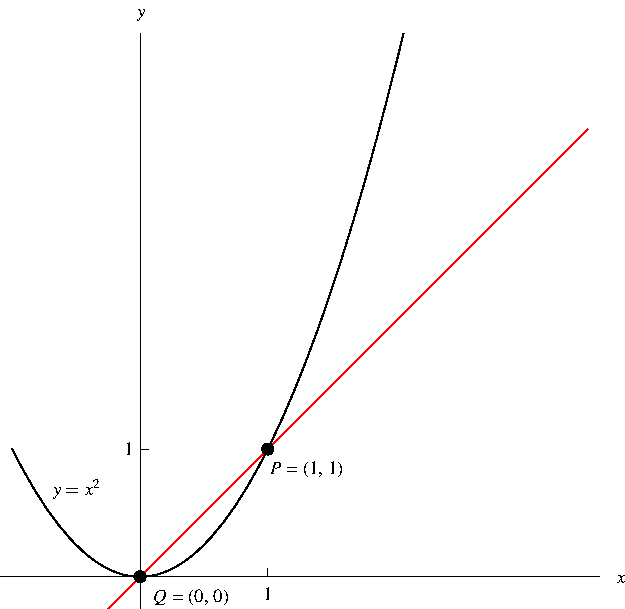
\includegraphics[height=5cm]{limits/pictures/02-01-secantg.pdf}%
%}%
%\only<handout:0| 19-20>{%
%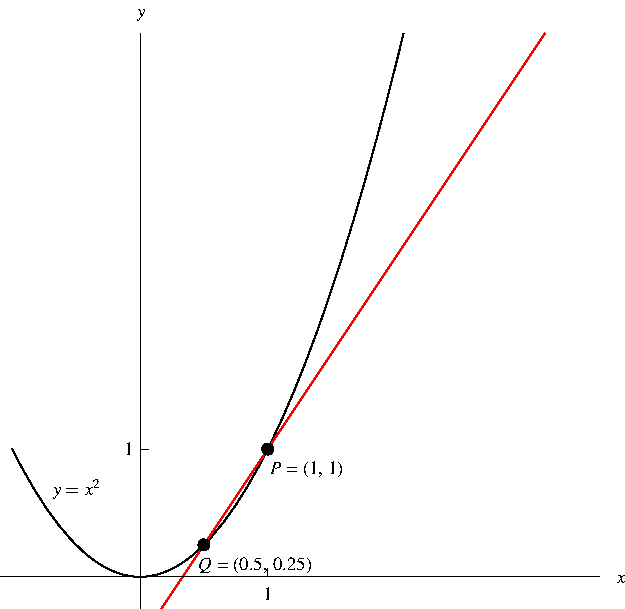
\includegraphics[height=5cm]{limits/pictures/02-01-secanth.pdf}%
%}%
%\only<handout:0| 21-22>{%
%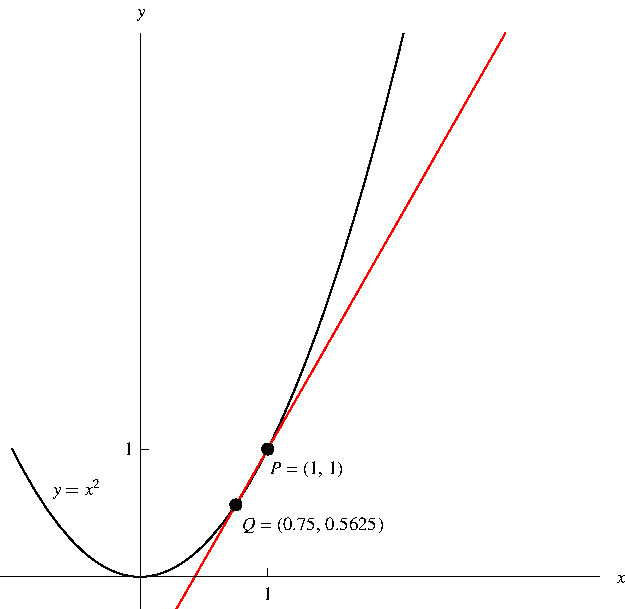
\includegraphics[height=5cm]{limits/pictures/02-01-secanti.pdf}%
%}%
%\only<handout:3| 23->{%
%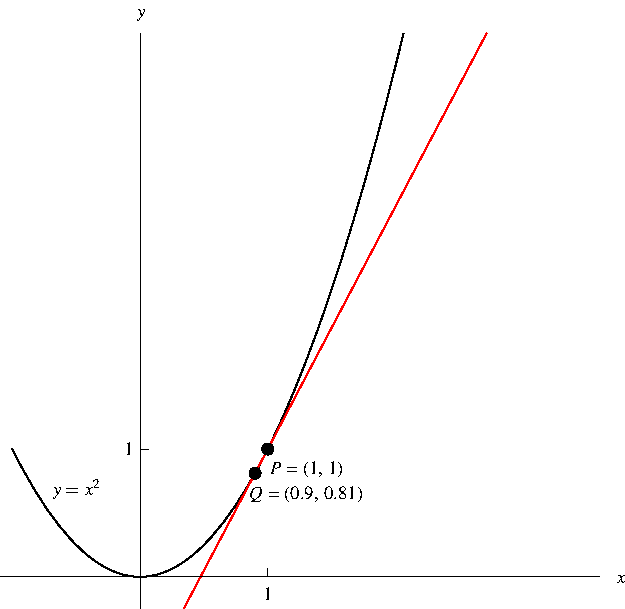
\includegraphics[height=5cm]{limits/pictures/02-01-secantj.pdf}%
%}%
\[
\begin{array}{|r@{}c@{}l|r@{}c@{}l||r@{}c@{}l|r@{}c@{}l|}
\hline
\multicolumn{3}{|c|}{x} &
\multicolumn{3}{|c||}{m_{PQ}} &
\multicolumn{3}{|c|}{x} &
\multicolumn{3}{|c|}{m_{PQ}} \\
\hline
\alert<handout:2| 7-8>{2} & & &
\uncover<handout:2-| 8->{\alert<handout:2| 8>{3}} & & &
\alert<handout:0| 17-18>{0} & & &
\uncover<handout:3| 18->{\alert<handout:0| 18>{1}} & & \\
\alert<handout:0| 9-10>{1} & 
\alert<handout:0| 9-10>{.} &
\alert<handout:0| 9-10>{5} &
\uncover<handout:3| 10->{\alert<handout:0| 10>{2}} & 
\uncover<handout:3| 10->{\alert<handout:0| 10>{.}} & 
\uncover<handout:3| 10->{\alert<handout:0| 10>{5}} &
\alert<handout:0| 19-20>{0} & 
\alert<handout:0| 19-20>{.} &
\alert<handout:0| 19-20>{5} &
\uncover<handout:3| 20->{\alert<handout:0| 20>{1}} & 
\uncover<handout:3| 20->{\alert<handout:0| 20>{.}} & 
\uncover<handout:3| 20->{\alert<handout:0| 20>{5}} \\
\alert<handout:0| 11-12>{1} & 
\alert<handout:0| 11-12>{.} &
\alert<handout:0| 11-12>{25} &
\uncover<handout:3| 12->{\alert<handout:0| 12>{2}} & 
\uncover<handout:3| 12->{\alert<handout:0| 12>{.}} & 
\uncover<handout:3| 12->{\alert<handout:0| 12>{25}} &
\alert<handout:0| 21-22>{0} & 
\alert<handout:0| 21-22>{.} &
\alert<handout:0| 21-22>{75} &
\uncover<handout:3| 22->{\alert<handout:0| 22>{1}} & 
\uncover<handout:3| 22->{\alert<handout:0| 22>{.}} & 
\uncover<handout:3| 22->{\alert<handout:0| 22>{75}} \\
\alert<handout:0| 13-14>{1} & 
\alert<handout:0| 13-14>{.} &
\alert<handout:0| 13-14>{1} &
\uncover<handout:3| 14->{\alert<handout:0| 14>{2}} & 
\uncover<handout:3| 14->{\alert<handout:0| 14>{.}} & 
\uncover<handout:3| 14->{\alert<handout:0| 14>{1}} &
\alert<handout:3| 23-24>{0} & 
\alert<handout:3| 23-24>{.} &
\alert<handout:3| 23-24>{9} &
\uncover<handout:3| 24->{\alert<handout:3| 24>{1}} & 
\uncover<handout:3| 24->{\alert<handout:3| 24>{.}} & 
\uncover<handout:3| 24->{\alert<handout:3| 24>{9}} \\
\alert<handout:0| 15-16>{1} & 
\alert<handout:0| 15-16>{.} &
\alert<handout:0| 15-16>{01} &
\uncover<handout:3| 16->{\alert<handout:0| 16>{2}} & 
\uncover<handout:3| 16->{\alert<handout:0| 16>{.}} & 
\uncover<handout:3| 16->{\alert<handout:0| 16>{01}} &
\alert<handout:0| 25-26>{0} & 
\alert<handout:0| 25-26>{.} &
\alert<handout:0| 25-26>{99} &
\uncover<handout:3| 26->{\alert<handout:0| 26>{1}} & 
\uncover<handout:3| 26->{\alert<handout:0| 26>{.}} & 
\uncover<handout:3| 26->{\alert<handout:0| 26>{99}} \\
\hline
\end{array}
\]
\column{.6\textwidth}
\begin{itemize}
\item  Find the tangent to $y = x^2$ at $(1,1)$.
\item<2->  Tangent has equation $y - 1 = m(x - 1)$, where $m$ is its slope.
\item<3->  If we know the slope, we know the line.
\item<4->  If we know two points, we can find the slope. We know one point, $P$; we need another point.
\item<handout:2-| 5->  Choose a nearby point $Q = (x, x^2)$ on the parabola and find the slope $m_{PQ}$ of the secant line $PQ$.
\item<handout:3-| 27->  The closer $x$ is to $1$, the closer $m_{PQ}$ is to $2$.
\item<handout:3-| 28->  This suggests the slope of the tangent should be $2$.
\end{itemize}
\end{columns}
\end{frame}
% end module tangent-problem
